% !TeX root = main.tex
\documentclass[11pt,a4paper]{article}
% \documentclass[a4paper,14pt, draft]{article}

%%% отключение нумерации сраниц
\pagestyle{empty}
%%% значок в itemize
% \renewcommand{\labelitemi}{$\cdot$}

%%% Работа с русским языком
\usepackage{cmap}					% поиск в PDF
\usepackage{mathtext} 				% русские буквы в формулах
\usepackage[T1, T2A]{fontenc}			% кодировка %Т1 посоветовал чат гпт
\usepackage[utf8]{inputenc}			% кодировка исходного текста
\usepackage[english,russian]{babel}	% локализация и переносы
\usepackage{indentfirst}            % красная строка в первом абзаце
\frenchspacing                      % равные пробелы между словами и предложениями

%%% Дополнительная работа с математикой
\usepackage{amsmath,amsfonts,amssymb,amsthm,mathtools} % пакеты AMS
\usepackage{icomma}                                    % "Умная" запятая

%%% Свои символы и команды
\usepackage{centernot} % центрированное зачеркивание символа
\usepackage{stmaryrd}  % некоторые спецсимволы
\usepackage{dsfont}
\usepackage{amsthm}


\renewcommand{\epsilon}{\ensuremath{\varepsilon}}
\renewcommand{\phi}{\ensuremath{\varphi}}
\renewcommand{\kappa}{\ensuremath{\varkappa}}
\renewcommand{\le}{\ensuremath{\leqslant}}
\renewcommand{\leq}{\ensuremath{\leqslant}}
\renewcommand{\ge}{\ensuremath{\geqslant}}
\renewcommand{\geq}{\ensuremath{\geqslant}}
\renewcommand{\emptyset}{\ensuremath{\varnothing}}

\DeclareMathOperator{\sgn}{sgn}
\DeclareMathOperator{\ke}{Ker}
\DeclareMathOperator{\im}{Im}
\DeclareMathOperator{\re}{Re}

\newcommand{\N}{\mathbb{N}}
\newcommand{\Z}{\mathbb{Z}}
\newcommand{\Q}{\mathbb{Q}}
\newcommand{\R}{\mathbb{R}}
\newcommand{\Cm}{\mathbb{C}}
\newcommand{\F}{\mathbb{F}}
\newcommand{\id}{\mathrm{id}}
\newcommand{\imp}[2]{
	(#1\,\,$\ra$\,\,#2)\,\,
}
\newcommand{\Root}[2]{
	\left\{\!\sqrt[#1]{#2}\right\}
}
\newcommand{\RR}{\R}
\newcommand{\NN}{\N}
\renewcommand{\subseteq}{\subset}
\newcommand{\sub}{\subset}
\newcommand{\sconstr}{\;\vert\;}
\newcommand{\thus}{\implies}

\newcommand{\defeq}{\vcentcolon= }
\newcommand{\defev}{\stackrel{\Delta}{\Longleftrightarrow}}
\newcommand{\deriv}[3][1]{%
	\ifthenelse{#1>1}{%
		\frac{\dlta^{#1} {#2}}{\dlta {#3}^{#1}}
	}{%
		\frac{\dlta {#2}}{\dlta {#3}}
	}%
}

\renewcommand\labelitemi{$\triangleright$}

\let\bs\backslash
\let\lra\Leftrightarrow
\let\ra\Rightarrow
\let\la\Leftarrow
\let\emb\hookrightarrow

%%% Перенос знаков в формулах (по Львовскому)
\newcommand{\hm}[1]{#1\nobreak\discretionary{}{\hbox{$\mathsurround=0pt #1$}}{}}

%%% Работа с картинками
\usepackage{graphicx}    % Для вставки рисунков
\setlength\fboxsep{3pt}  % Отступ рамки \fbox{} от рисунка
\setlength\fboxrule{1pt} % Толщина линий рамки \fbox{}
\usepackage{wrapfig}     % Обтекание рисунков текстом

% \usepackage[inkscapeformat=png]{svg} %% svg

%%% Работа с таблицами
\usepackage{array,tabularx,tabulary,booktabs} % Дополнительная работа с таблицами
\usepackage{longtable}                        % Длинные таблицы
\usepackage{multirow}                         % Слияние строк в таблице

%%% Теоремы
\theoremstyle{plain}
\newtheorem*{theorem}{Теорема}
\newtheorem*{lemma}{Лемма}
\newtheorem*{proposition}{Утверждение}
\newtheorem*{exercise}{Упражнение}
\newtheorem*{problem}{Задача}

\theoremstyle{definition}
\newtheorem*{definition}{Определение}
\newtheorem*{corollary}{Следствие}
\newtheorem*{note}{Замечание}
\newtheorem*{reminder}{Напоминание}
\newtheorem*{example}{Пример}

\theoremstyle{remark}
\newtheorem*{solution}{Решение}

%%% Оформление страницы
\usepackage{extsizes}     % Возможность сделать 14-й шрифт
\usepackage{geometry}     % Простой способ задавать поля
\usepackage{setspace}     % Интерлиньяж
\usepackage{enumitem}     % Настройка окружений itemize и enumerate
\setlist{leftmargin=10pt} % Отступы в itemize и enumerate

\geometry{top=15mm}    % Поля сверху страницы
\geometry{bottom=5mm} % Поля снизу страницы
\geometry{left=10mm}   % Поля слева страницы
\geometry{right=10mm}  % Поля справа страницы

\setlength\parindent{15pt}        % Устанавливает длину красной строки 15pt
\linespread{1}                  % Коэффициент межстрочного интервала
%\setlength{\parskip}{0.5em}      % Вертикальный интервал между абзацами
\setcounter{secnumdepth}{0}      % Отключение нумерации разделов
%\setcounter{section}{-1}         % Нумерация секций с нуля
\usepackage{multicol}			  % Для текста в нескольких колонках
\usepackage{soulutf8}             % Модификаторы начертания
\mathtoolsset{showonlyrefs=true} % показывать номера формул только у тех, у которых есть ссылки по eqref
%%% Содержаниие
% \usepackage{tocloft}
% \tocloftpagestyle{main}
%\setlength{\cftsecnumwidth}{2.3em}
%\renewcommand{\cftsecdotsep}{1}
%\renewcommand{\cftsecpresnum}{\hfill}
%\renewcommand{\cftsecaftersnum}{\quad}

%%% Нумерация уравнений
\makeatletter
\def\eqref{\@ifstar\@eqref\@@eqref}
\def\@eqref#1{\textup{\tagform@{\ref*{#1}}}}
\def\@@eqref#1{\textup{\tagform@{\ref{#1}}}}
\makeatother                      % \eqref* без гиперссылки
\numberwithin{equation}{section}  % Нумерация вида (номер_секции).(номер_уравнения)
\mathtoolsset{showonlyrefs= true} % Номера только у формул с \eqref{} в тексте.

%%% Гиперссылки
\usepackage{hyperref}
\usepackage[usenames,dvipsnames,svgnames,table,rgb]{xcolor}
\hypersetup{
	unicode=true,            % русские буквы в раздела PDF
	colorlinks=true,       	 % Цветные ссылки вместо ссылок в рамках
	linkcolor=black!15!blue, % Внутренние ссылки
	citecolor=green,         % Ссылки на библиографию
	filecolor=magenta,       % Ссылки на файлы
	urlcolor=NavyBlue,       % Ссылки на URL
}

%%% Графика
\usepackage{tikz}        % Графический пакет tikz
\usepackage{tikz-cd}     % Коммутативные диаграммы
\usepackage{tkz-euclide} % Геометрия
\usepackage{stackengine} % Многострочные тексты в картинках
\usetikzlibrary{angles, babel, quotes}
%%% значок в itemize
\renewcommand{\labelitemi}{$\multimap  $}
\title{\texttt{Получение и измерение вакуума \\ 2.3.1}}
\author{}
\date{}

\begin{document}
\maketitle

\textbf{Цель работы:}
\begin{itemize}
  \item Измерение объёмов форвакуумной и высоковакуумной частей установки
  \item  Определение скорости откачки системы в
        стационарном режиме, а также по ухудшению и по улучшению вакуума.
\end{itemize}

\textbf{В работе используются:} вакуумная установка с манометрами: масляным, термопарным и ионизационным.

\section*{\texttt{Теория}}
По степени разрежения вакуумные установки принято делить на
три класса: \begin{itemize}
  \item низковакуумные — до  $[10^{-2}; 10^{-3}]$ торр
  \item высоковакуумные — $[10^{-4}; 10^{-7}]$ торр
  \item установки сверхвысокого вакуума — $[10^{-8};10^{-11}]$ торр
\end{itemize}
С физической точки зрения низкий вакуум переходит в высокий, когда длина свободного
пробега молекул газа оказывается сравнима с
размерами установки (а течение газа становится сугубо молекулярным).
Cверхвысокий вакуум характерен крайней важностью
процессов адсорбции и десорбции частиц на поверхности вакуумной камеры.
\\ Формула диффузии:
\[\frac{dN}{dt} = D\frac{dn}{dx}S\]
$D = \frac{\lambda \overline v}{3}, \lambda = 2r => D = 2r\overline v / 3\ \  (\overline v = \sqrt{\frac{8kT}{\pi m}})$
$\frac{dn}{dx} = \frac{n_1 - n_2}{L}$
\\ Формула Кнудсена:
\[\frac{dN}{dt} = \frac{4}{3}r^3\sqrt{\frac{2\pi kT}{m}}\frac{n_1 - n_2}{L}\]
Итоговая формула скорости убвания массы:
\[\frac{dM}{dt} = \frac{4}{3}\fbox{$r^3$}\sqrt{\frac{2\pi \mu}{RT}}\frac{P_1-P_2}{l}\]
Формула Пуазейля для сплошной среды:
\[\frac{dM}{dt} = \frac{3\pi}{32}\frac{\fbox{$r^4$}}{\lambda}\sqrt{\frac{2\pi m}{kT}}\frac{P_1 - P_2}{L}\]
\\
Основное отличие формул для расхода газа, имеющего свойства
сплошной среды, и в случае очень разреженного газа в том, что рас-
ход сплошной среды пропорционален $r^4$, а разреженной — только
$r^3$\\
\\
На границе раздела фаз силы межмолекулярного взаимо-
действия не скомпенсированы из-за разной плотности вещества, и
поэтому пограничный слой обладает избытком энергии. Поглощение какого-либо
вещества из газообразной среды или раствора поверхностным слоем
жидкости или твёрдого тела называется \textbf{адсорбцией}.


\section*{Экспериментальная установка}
\subsection*{\texttt{Важные константы:}}
\begin{itemize}
  \item
\end{itemize}

В данной работе изучаются традиционные методы откачки
механическим форвакуумным насосом до давления
$10^{-2}$ торр и диффузионным
масляным насосом до давления $10^{-5}$ торр, а также методы измерения
вакуума в этом диапазоне.
\begin{figure}[h!]
  \includegraphics*[width=\textwidth]{ust.png}
  \caption{Схема экспериментальной установки}
  \label{fig:ust}
\end{figure}
\begin{figure}[h!]
  \includegraphics*[width=\textwidth]{ust2.png}
  \caption{Схема действия ротационного двухпластинчатого форвакуумного на-
    соса. В положениях «а» и «б» пластина «А» засасывает разреженный воздух
    из откачиваемого объёма, а пластина «Б» вытесняет ранее захваченный воз-
    дух в атмосферу. В положениях «в» и «г» пластины поменялись ролями}
  \label{fig:ust2}
\end{figure}
\begin{figure}[h!]
  \includegraphics*[width=\textwidth]{ust3.png}
  \caption{Схема работы диффузионного насоса}
  \label{fig:ust3}
\end{figure}
% \noindent Схема экспериментальной установки представлена на рис~\ref{fig:ust}.

Измеряем пройденное расстояние линейкой, а время -- секундомером,
находим $v_\text{уст}$. Радиус шарика измеряем горизонтальным
компаратором/микроскопом (для каждого шарика измеряем насколько диаметров и берём среднее).
Плотность шариков и жидкости -- табличные значения.\\
Опыты проводятся при нескольких температурах в интервале от
комнатной до $320-330$ К.\\
Для каждой температуры проводим измерения с разными диаметрами шариков.\\
Построим график в координатах $ln\eta (T^{-1})$.\\
Если во всем диапазоне встречающихся в работе
скоростей и времён релаксации вычисленные по нашей формуле
значения $\eta$ оказываются одинаковыми, то формула Стокса правильно
передаёт зависимость сил от радиуса шарика.
Если всё-таки наблюдается кореляция $\eta$ и $r$, то нужно использовать формулу:
\begin{center}{
    \fbox{
      $\eta = \frac{2}{9}gr^2\frac{\rho - \rho_\text{ж}}{v_\text{уст}} \cdot \frac{1}{1 + 2.4(r/R)}$
    }}\end{center}
где R --  радиус сосуда.

\section*{Ход работы}
\subsection*{Определение объёма форвакуумной и высоковакуумной
частей установки}
\begin{enumerate}
  \setcounter{enumi}{-1}
  \item Проверим, что все краны в правильном положени.
  \item Откроем кран, подождём несколько минут пока воздух заполнит установку
  \item Откачаем форвакуумным насосом воздух до давления порядка $10^{-2}$ торр.
  \item Впустим воздух в форвакуумную часть установки и измерим давление.
  \item Отсоединим установку от форвакуумного насоса, откроем на всю форвакуумную часть
 в краны и капилляры.
 
  \item Зафиксируем давление. Высота масла в манометре: 
   \[ h_1 = (38.4 \pm 0.2)\text{см},\  h_2 = (11.6 \pm 0.2) \text{см} => \Delta h_\text{фв} = (26.8 \pm 0.3) \text{см}\]
  \begin{align}
    \sigma_{\Delta h} = \sqrt{\sigma_{h1}^2 + \sigma_{h2}^2}\approx 0.3 \text{см} => \varepsilon_{\Delta h} = 1 \ \% 
  \end{align}
  
  
  \item $V_\text{закртой} = 50 \text{см}^3$, используем $\Delta P V_\text{закрытой}=P_2 V_2$ вычислим объем форвакуумной части установки. 
  При этом давление $P_1 = P_\text{атм} = 100 \text{кПа}$, а относительная погрешность полученного 
  значения равна относительной погрешности величины $\Delta h_\text{фв} $:
  \[\Delta P = \rho_\text{масл} g \Delta h_\text{фв} = 2.33 \ \text{кПа}, \ \ \  \rho_\text{масл} = 885 \ \frac{\text{кг}}{\text{м}^3}\]
  
  \begin{equation}
    V_\text{фв} = \frac{P_1 V_\text{закрытой}}{P_2} - V_\text{закрытой} = 2.1 \ \text{л}
  \end{equation}
  

  \item Аналогично с диффузионным насосом, но нужно будет вычесть объем форвакуумной части. 
 \[
    h_3 = (33.5 \pm 0.2) \text{см}, h_4 = (16.6 \pm 0.2) \text{см} => \Delta h_{полн} = (16.9 \pm 0.3) \text{см}.
\]

  
  Аналогично погрешности высот:
  \begin{align}
    V_\text{полн} = \frac{P_1}{\rho g \Delta h_\text{полн}} V_{кап} \approx 3.4\text{л},&&
    \varepsilon_{V_{полн}} = \varepsilon_{\Delta h} \approx 2~\%.
  \end{align}
  
  Тогда объём высоковакуумной части:
  \[
    V_\text{вв} = V_\text{полн} - V_\text{фв} = 1.3\text{л}, \sigma_{V_\text{вв}} = \sqrt{\sigma_{V_\text{полн}}^2+ \sigma_{V_\text{фв}}^2} = 0.07 \approx 0.1\text{л},
  \]
\end{enumerate}
	\begin{enumerate}
		% \setcounter{enumi}{7}
		
		\item Не выключая форвакуумного насоса убедимся в том, что в установке не осталось запертых объемов. 
		
		\item Откачав установку до давления порядка $ 10^{-2}~торр$, приступим к откачке ВБ с помощью диффузионного насоса. 
		
		
		\item С помощью термопарного манометра пронаблюдаем за тем, как идет откачка ВБ. Мы должны продолжать процесс откачки до тех пор, пока там не установится давление порядка $10^{-4}~\text{торр}.$ 
		
		\item С помощью ионизационного манометра измерим значение предельного давления в системе со стороны высоковакуумной части: $$P_\text{пр} = (6.1 \pm 0.1)  \cdot 10^{-5} ~\text{торр}.$$
		
		
		\item Найдем скорость откачки по ухудшению и улучшению вакуума, для этого открывая и закрывая кран $K_3$ будем то подключать насос к объему, то отключать его, при этом на видео зафиксируем показания манометра от времени и построим графики необходимых  зависимостей (каких именно подробнее описано в соответствующих пунктах ниже), для которых определим коэффициенты наклона прямых и их погрешности (с помощью МНК).
		
		Для случая улучшения вакуума воспользуемся формулой \eqref{exp} и построим график зависимости $-(ln(P-P_\text{пр}))$ от $t$. При построении такого графика из МНК получим коэффициент наклона --- $k$, с помощью которого можно найти $W = kV_\text{вв}$. Построим эти графики:	
		\begin{figure}[h!]
			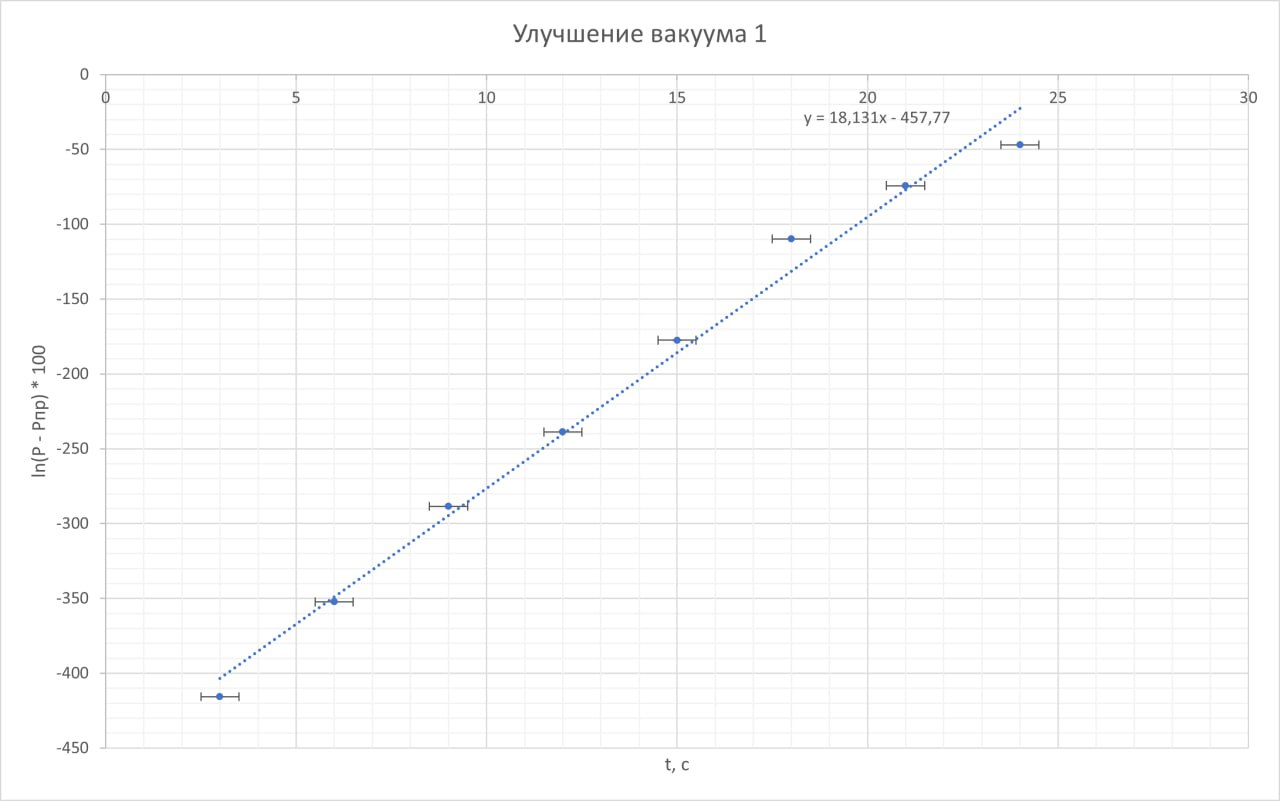
\includegraphics[scale=1.6]{IncreaseVacuum1}
			\caption{Улучшение вакуума 1}
			\label{graph2}
		\end{figure}
		\bgroup
		\def\arraystretch{1.3}%
		\begin{table}
			\begin{center}
				\begin{tabular}{|c|c|c|c|c|}
					\hline
					$k \cdot 10^{-1},~\frac{1}{с}$ & $\sigma_k^{сл} \cdot 10^{-1},~\frac{1}{с}$ & $W \cdot 10^{-1},~\frac{л}{с}$ & $\varepsilon_W$ & $\sigma_W \cdot 10^{-1},~\frac{л}{с}$\\
					\hline
					1.81& 0.07 & 2.4 & 7 \% & 0.2\\
					\hline
					1.82&0.03 & 2.4 & 6 \% & 0.1 \\
					\hline
				\end{tabular}
			\end{center}
			\caption{Коэффициенты наклона при улучшении вакуума}
			\label{tab1}
		\end{table}
		\egroup
		\item Оценим величину потока газа  $Q_H$. Для этого воспользуемся данными, полученными при ухудшении вакуума. А именно построим графики зависимости $P(t)$ и определим для них коэффициенты угла наклона прямой. Примем погрешность показаний термопарного манометра за $2 \%$ в среднем.
     Поскольку $V_\text{вв}dP = (Q_\text{Д} + Q_\text{И}) dt$ получим $(Q_\text{Д} + Q_\text{И}) = \alpha V_\text{вв}$. По графикам получаем:
		\bgroup
		\def\arraystretch{1.3}%
		\begin{table}[h!]
			\begin{center}
				\begin{tabular}{|c|c|c|c|c|c|}
					\hline
					$\alpha \cdot 10^{-6},~\frac{торр}{с}$ & $\sigma_{\alpha}^{сл}\cdot 10^{-6},~\frac{торр}{с}$& $\varepsilon_{\alpha}$ &$\sigma_{\alpha}\cdot^{-6},~\frac{торр}{с}$&  $Q_{д}+Q_{и},~торр\cdot\frac{л}{с}$ & $\sigma_{Q_{д}+Q_{и}},~торр\cdot\frac{л}{с}$\\
					\hline
					8.9& 0.05 & 2.1 \% & 0.2 & $1.16\cdot10^{-5}$& {$0.07\cdot10^{-5}$}\\
					\hline
					8.1&0.04&2.1& 0.2 & $1.05\cdot10^{-5}$ & {$0.06\cdot10^{-5}$} \\
					\hline
				\end{tabular}
			\end{center}
			\caption{Коэффициенты наклона при ухудшении вакуума}
			\label{tab2}
		\end{table}
		\egroup
		\begin{figure}[h!]
			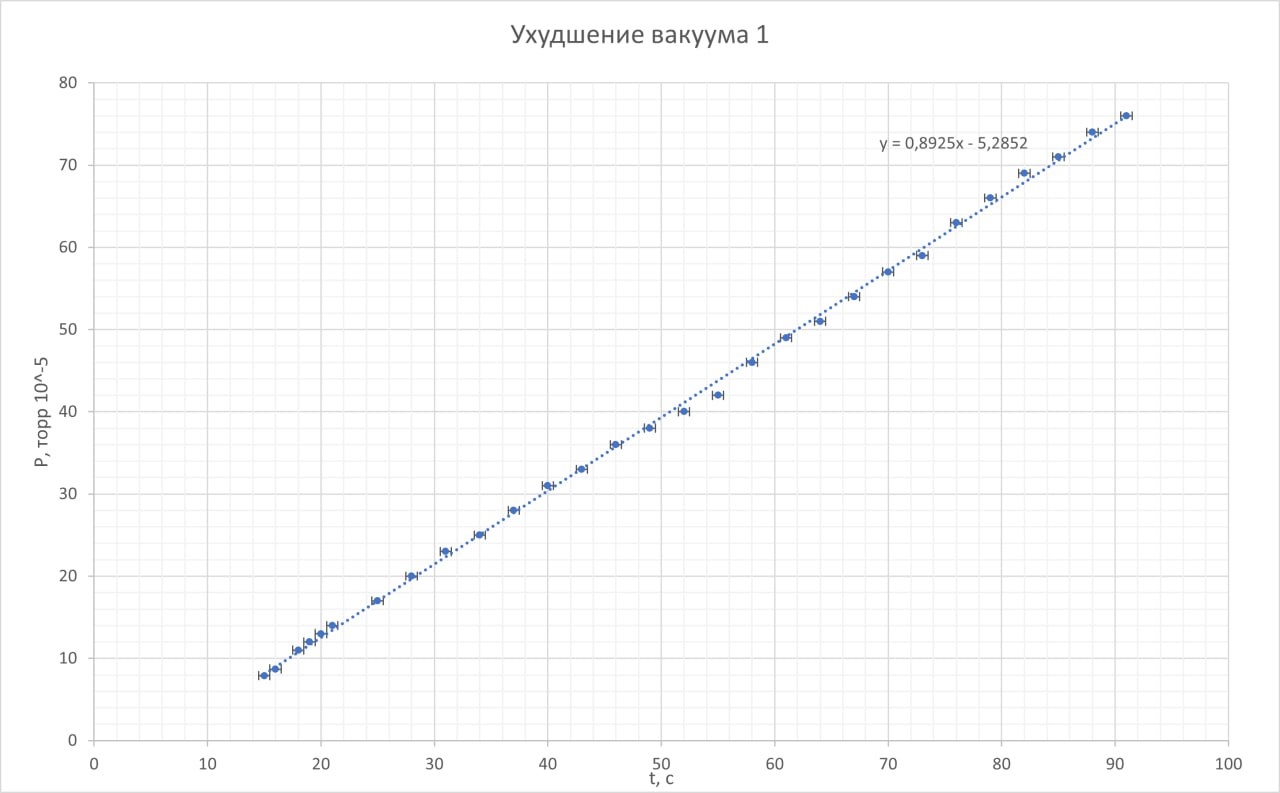
\includegraphics[scale=1.6]{DecreaseVacuum1}
			\caption{Ухудшение вакуума 1}
			\label{graphup1}
		\end{figure}
		Используя формулу $Q_\text{Н} = P_\text{пр}W - (Q_\text{Д} + Q_\text{И})$, а значит $\sigma_{Q_\text{Н}} =  \sqrt{\sigma_{P_\text{пр}W}^2 + \sigma^2} \approx 1.1 \cdot 10^{-6}$ получим, что: $Q_H = (3.6 \pm 1.1) \cdot 10^{-6} \text{торр} \cdot \text{л} / \text{с}.$
		
		\newpage
		\item Параметры трубки:
			$$L = 10.8~ \text{см},  d = 0.8 ~ \text{мм},$$
		
		
		\item Введем в систему искусственную течь и запишем значение  установившегося при этом давления и давления $P_{фв}$: 
		
		\begin{align}
			P_{\text{уст}} = (9.1 \pm 0.1) \cdot 10^{-5} ~ \text{торр}. && P_{фв} = (1.0 \pm 0.1) \cdot 10^{-4} ~ \text{торр}.
		\end{align}
		
		
		\item Поскольку
		$$P_\text{пр} W = Q_1, \quad P_\text{уст} W = Q_1 + \frac{d(PV)_\text{закрытой}}{dt},$$
		то с учетом \eqref{ty}, получаем:
		\begin{equation}
			W = \frac{P_\text{фв}}{P_\text{уст}-P_\text{пр}}\frac{4r^3}{3L}\sqrt{\frac{2\pi RT}{\mu}} \approx 0.167 \cdot 10^{-2}~\frac{\text{л}}{\text{с}}
		\end{equation}
		
		\item Следуя указаниям в методичке выключаем установку.
		
	\end{enumerate}
	 

	\section{Вывод}
	\begin{itemize}
		\item Измерили объемы форвакуумной, высоковакуумной части установки, так же как и объем всей установки.
		
		\item Определили скорость откачки двумя способами.
		
		Возможными причинами расхождения полученных результатов на один порядок могло послужить изменение температуры, созданное нагреваемым масляным высоковакуумным насосом. Также возможна разница из-за принципа работы высоковакуумного насоса -- при уменьшении давления в нем, производительность начинает падать.
		
		\item Оценили поток газа, поступающего из насоса в откачиваемую систему.
		
		
		
		
	\end{itemize}
	
	\newpage
	
	\section{Графики}
	
	\centering
	\begin{figure}[h!]
		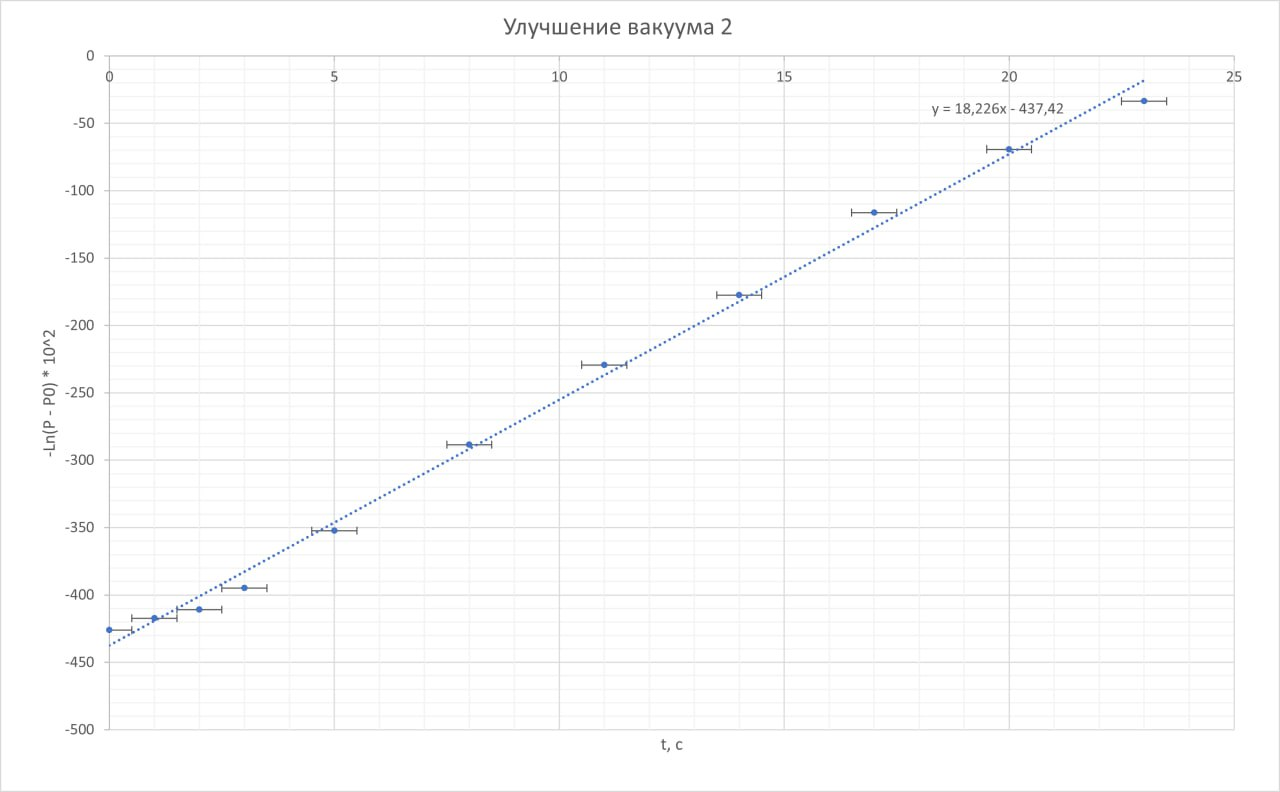
\includegraphics[scale=1.6]{IncreaseVacuum2}
		\caption{Улучшение вакуума 2}
		\label{graph3}
	\end{figure}
	
	\begin{figure}[h!]
		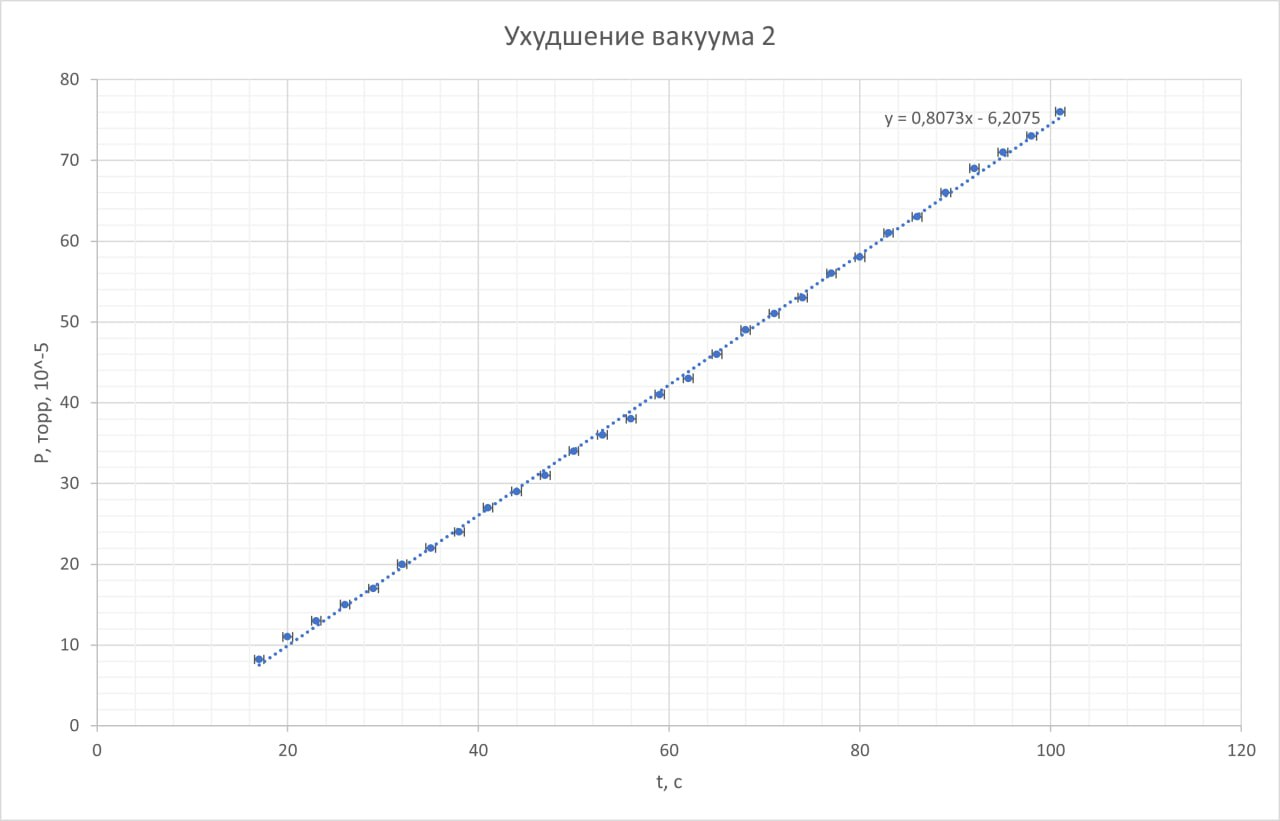
\includegraphics[scale=1.6]{DecreaseVacuum2}
		\caption{Ухудшение вакуума 2}
		\label{graph4}
	\end{figure}
	
\end{document}